\documentclass[paper=a4,fontsize=10pt,jafontsize=10pt,line_length=44zw,number_of_lines=46]{jlreq}
\usepackage{amsmath,amssymb,graphicx,booktabs,multirow,siunitx,xcolor}
\usepackage[hidelinks]{hyperref}
\newcommand{\tauh}{\tau_{\mathrm{h}}}
\newcommand{\taul}{\tau_{\ell}}
\newcommand{\abinv}{\,\mathrm{ab}^{-1}}
\newcommand{\fbinv}{\,\mathrm{fb}^{-1}}
\newcommand{\hvec}{\boldsymbol{h}}
\newcommand{\phicp}{\varphi^{*}_{CP}}

\title{学習した$\tau$偏極計による$H\to\tau\tau$のスピン状態の測定：\\HL-LHCにおける$\tau$湯川結合のCP混合角と$\tau$対のスピンもつれ}
\author{（著者名）\\（所属）}
\date{2026年10月}

\begin{document}
\maketitle

\begin{abstract}
$H\to\tau^+\tau^-$崩壊の$\tau$対のスピン状態は，$\tau$湯川結合のCP性質を決め，同時に量子もつれの検証の対象にもなる．しかし$\tau$崩壊のニュートリノが失われるため，ハドロン衝突型加速器でスピン状態を測ることは難しいとされてきた．本論文では，一次頂点を基準にした衝突径数と二次頂点を$\tau$の局所座標で表して偏極計ベクトルを回帰する手法（tauspin）を用い，HL-LHC（$\sqrt s=14$\,TeV，$3\abinv$，1実験，$\tauh\tauh$チャンネル）で$H\to\tau\tau$のスピン状態がどこまで測れるかを見積もる．スピン無偏極で崩壊させた試料の厳密な再重み付けでテンプレートを作り，背景のスピン分布は$m_{\tau\tau}$の側帯で決める（またはその分布を補助試料で拘束する），分離可能な全てのBell対角状態を帰無仮説とする，といった頑健な尤度で評価した．tauspinは，LHCのCP解析で用いられる観測量（零運動量系での$\phicp$）と教科書的な観測量を最適に組み合わせたものに対し，CP混合角$\varphi_\tau$の期待精度で$\pm13.9^\circ$対$\pm19.0^\circ$（背景のスピン分布を側帯で決める場合）と$\pm7.2^\circ$対$\pm9.9^\circ$（既知の場合），もつれの期待有意度で$1.84\sigma$対$1.36\sigma$（同）と$3.51\sigma$対$2.61\sigma$を与え，感度は一貫して$1.35$〜$1.37$倍，ルミノシティに換算して約$1.8$〜$1.9$倍になる．情報の削除実験から，この利得の大部分は横方向の衝突径数に由来することが分かる．一方，もつれの確立は1実験では背景分布を補助試料で拘束しても約$3\sigma$にとどまり，さらに横方向の解析力の独立な較正を必要とする．CP混合角の精度は解析力の全体スケールには頑健である．
\end{abstract}

\section{序論}

Higgs粒子と$\tau$レプトンの湯川結合は，CP偶の成分とCP奇の成分の混合角$\varphi_\tau$で
\begin{equation}
  \mathcal L_{H\tau\tau}\propto -\frac{m_\tau}{v}\,\kappa_\tau\,\bar\tau\left(\cos\varphi_\tau+i\gamma_5\sin\varphi_\tau\right)\tau\,H
\end{equation}
とパラメータ化できる．標準模型は$\varphi_\tau=0$であり，0でない値は新しいCP対称性の破れを意味する．$\varphi_\tau$は$\tau$対のスピン相関に現れ，ATLASとCMSはRun~2のデータで$\varphi_\tau=9\pm16^\circ$\cite{ATLAS:2022akr}，$-1\pm19^\circ$\cite{CMS:2021sdq}を測定した（期待精度はそれぞれ$\pm28^\circ$と約$\pm21^\circ$）．これらの解析は，$\tau$の崩壊生成物の作る面の間の角度$\phicp$\cite{Berge:2008dr,Berge:2015nua}を，衝突径数（IP）法や$\rho$崩壊面の方法で構成している．

同じスピン相関は量子もつれの検証にも使える．スカラー粒子から生じる$\tau$対は，理想的には最大もつれのBell状態にある．LHCでは$t\bar t$対のスピンもつれがATLASとCMSで観測され\cite{ATLAS:2023fsd,CMS:2024pts,Afik:2020onf}，衝突型加速器での量子情報の研究が盛んになっている．$H\to\tau\tau$のもつれやBell不等式は主に将来の電子・陽電子衝突型加速器で提案されてきた\cite{Altakach:2022ywa,Fabbrichesi:2022ovb,Ma:2023yvd}．欧州戦略の量子情報に関する入力文書\cite{QI:ESPPU}は，ニュートリノのためLHCでの$H\to\tau\tau\to\pi\nu\pi\nu$によるもつれの研究は不可能か著しく困難であると述べている．一方，$Z/\gamma^*\to\tau\tau$でのもつれの研究はLHCでも提案されている\cite{ZttEnt}．

ハドロン衝突型加速器での最大の障害は，失われたニュートリノのために$\tau$の静止系と偏極計ベクトル$\hvec$が正確に再構成できないことである．これまでに，IPと質量殻条件による$\tau$運動量の再構成\cite{Hagiwara:2016zqz,HtautauCPV}や，深層学習による$\varphi_\tau$の推定\cite{Jozefowicz:2016kvz,Lasocha:2020ctd,Lasocha:2024}が提案されているが，多くは生成器水準と簡易な分解能での評価である．

著者らは先行研究（tauspin，未発表）で，一次頂点（PV）基準のIPと二次頂点（SV）を$\tau$の局所座標で表し，偏極計ベクトルそのものを機械学習で回帰する手法を開発した．ATLASの完全シミュレーションで，同じ質量の$H$と$Z$を$\tau\tau$のスピンだけで区別するAUCが$0.626$（正確な偏極計で約$0.72$〜$0.73$）に達し，IPが可視粒子と欠損運動量だけでは決まらない$\tau$の方位角を約$2$\,mradの精度で測ることを示した．本論文では，この手法でHL-LHCの$H\to\tauh\tauh$のスピン状態がどこまで測れるかを，CP混合角ともつれの両方について見積もる．

本研究の特徴は三つある．第一に，検出器応答をtauspinのATLAS完全シミュレーションに較正した，検出器水準の評価である．第二に，CP混合角ともつれを同じ統計量の枠組みで扱い，LHCの実際のCP解析が用いる$\phicp$を比較の基準にする．第三に，背景のスピン分布をシミュレーションから取らずに$m_{\tau\tau}$の側帯で決め，帰無仮説を分離可能な状態の全体にとる頑健な尤度を用いる．背景分布を既知とし，Werner族の一点を帰無仮説とする簡略な評価では1実験で約$3.8\sigma$が得られるが，これらの仮定を外すと大きく下がる．本論文の数値は全て頑健な尤度によるものである．

\section{$\tau$対のスピン状態}\label{sec:spin}

\subsection{スピン密度と偏極計}

$\tau^\mp$の偏極計ベクトルを$\hvec^\mp$とすると，$\tau$対の崩壊分布は
\begin{equation}
  \rho(\hvec^-,\hvec^+)=1+\boldsymbol B^-\!\cdot\hvec^-+\boldsymbol B^+\!\cdot\hvec^++\sum_{ij}C_{ij}h^-_ih^+_j
\end{equation}
と書ける．各$\tau$の運動量方向$k$，$k$とビーム軸の張る面に垂直な$n$，残りの$r$からなる局所基底で，$\varphi_\tau$のHiggs粒子は
\begin{equation}
  \rho_{\varphi}=1-h^-_kh^+_k+\cos2\varphi\,(h^-_nh^+_n+h^-_rh^+_r)+\sin2\varphi\,(h^-_nh^+_r-h^-_rh^+_n)
  \label{eq:rhophi}
\end{equation}
となる．どの$\varphi$でも最大もつれ状態であり，CP偶とCP奇の違いは横方向の相関の「回転」として現れる．$Z\to\tau\tau$は$C_{kk}=+1$，$\tau$の縦偏極$P_\tau=-0.147$で，生成の仕方に応じた横方向の相関をもつ．

偏極計を実装した崩壊モードは$\pi$，$\rho$，$\pi2\pi^0$，$3\pi$である．$3\pi$の偏極計はPythia~8のCLEOハドロン流\cite{Bierlich:2022pfr}を移植して計算した．本論文の$H$+ジェット試料では，選別後の事象の$72\%$で両側の偏極計が定義される（$HH$試料では$71\%$\cite{dihiggs:paper}）．

\subsection{もつれの判定}

偏極をもたず，相関行列が対角な状態をBell対角状態と呼ぶ．Bell対角状態$\rho_{\boldsymbol c}=1+\sum_ic_ih^-_ih^+_i$は，$\boldsymbol c=(c_n,c_r,c_k)$が頂点$(1,1,-1)$，$(1,-1,1)$，$(-1,1,1)$，$(-1,-1,-1)$の四面体$\mathcal T$の中にあるとき物理的であり，八面体$\mathcal O=\{|c_n|+|c_r|+|c_k|\le1\}$の中にあるとき，かつそのときに限り分離可能である\cite{Horodecki:1996,Peres:1996dw}．CP偶のHiggs粒子は$\mathcal T$の頂点$(1,1,-1)$にある．$\mathcal T\setminus\mathcal O$で$(1,1,-1)$に面する部分の境界は$c_n+c_r-c_k=1$の面であり，$c_n+c_r-c_k>1$はもつれの十分条件であり，このような判定量をもつれの目撃者（witness）と呼ぶ．Bell状態と完全な無相関状態の混合であるWerner族$\boldsymbol c=p(1,1,-1)$では$p>1/3$がもつれに当たる\cite{Werner:1989zz}．

本論文のもつれの検定は，$\mathcal O$の全体を帰無仮説とし，$\mathcal T$の全体を対立仮説とする一般化尤度比である．これは量子力学を仮定し，$\tau$の崩壊をスピンの測定とみなしたうえでの「分離可能な状態の排除」であり，局所実在論の意味でのもつれの証明ではない\cite{Abel:2025,Bechtle:2025}．

\subsection{十分統計量}

スピン密度は$\boldsymbol c$や$\cos2\varphi$，$\sin2\varphi$について線形なので，測定量$x$の分布は
\begin{equation}
  p(x\mid\boldsymbol c)=p_0(x)\left[1+\sum_i c_i\,g_i(x)\right],\qquad g_i(x)=E_{\mathrm{flat}}\!\left[h^-_ih^+_i\,\middle|\,x\right]
\end{equation}
となる．ここで$E_{\mathrm{flat}}$はスピン無偏極の試料での条件付き期待値である．よって，もつれには$g_T=E_{\mathrm{flat}}[h^-_nh^+_n+h^-_rh^+_r|x]$と$g_L=E_{\mathrm{flat}}[h^-_kh^+_k|x]$，CP混合角には$g_T$と$g_A=E_{\mathrm{flat}}[h^-_nh^+_r-h^-_rh^+_n|x]$が（横方向の等方性のもとで）十分な統計量になる．これらを回帰で推定し，その2次元分布をテンプレートにする．

\section{シミュレーションと再構成}\label{sec:sim}

\subsection{試料}

Pythia~8.315\cite{Bierlich:2022pfr}内部の$gg/qg/q\bar q\to H$+ジェット（$\hat p_T>40$\,GeV，$m_H=125$\,GeV，$H\to\tau\tau$）を，$\tau$を無偏極・無相関に崩壊させて（\texttt{TauDecays:mode = 3}，偏極0）$1.5\times10^6$事象生成した．この「スピン平坦」試料の生成スピン密度は1なので，任意の仮説への重みは$\rho(\hvec)$そのもの（有界）であり，テンプレートは厳密に作れる（TauSpinner\cite{Czyczula:2012ny}と同じ考え方）．$b$タグを要求せず，二つの$\tauh$のpTを$40$，$30$\,GeV以上とする選別の後に$158{,}584$事象が残る．

検出器応答は，tauspinのATLAS完全シミュレーション検証試料で較正したパラメトリックな模型である（$\pi^0$のエネルギー・角度分解能，トラックの運動量分解能，崩壊モードの移行，$d_0$分解能$10\oplus150/p_T\,\mu$m，$z_0$分解能$20\oplus300/p_T\,\mu$m，SV分解能，欠損横運動量）．詳細は姉妹論文\cite{dihiggs:paper}に記した．

\subsection{再構成の水準}

統計量$g$は，次の入力から勾配ブースティング\cite{Pedregosa:2011}で回帰した（2分割の交差学習）．
\begin{description}
  \item[正確な$\hvec$] 真の偏極計（参照値）．
  \item[tauspin] PV基準のIPとSVを局所基底で表した入力から多層パーセプトロンで回帰した$\hat{\hvec}^\pm$と積$\widehat{h^-_ih^+_j}$，および再構成した崩壊モード．回帰器は等質量の$H(125)$+ジェットと$Z(125)$+ジェットで学習した（姉妹論文\cite{dihiggs:paper}）．
  \item[tauspin（IP・SVなし）] 同じ回帰器を，IPとSVの入力を除いて学習し直したもの．
  \item[tauspin（SV・IP縦成分・欠損運動量なし）] 横方向のIPと可視崩壊生成物だけで学習し直したもの（情報の削除実験）．
  \item[LHCのCP観測量] ATLASとCMSのCP解析と同じ$\phicp$．荷電トラックの零運動量系で，$1$本トラック・$\pi^0$なしと3本トラックには先頭トラックのIPベクトル，$\pi^0$を伴う崩壊には$\rho$崩壊面を用い，$y=(E_{\pi^\pm}-E_{\pi^0})/(E_{\pi^\pm}+E_{\pi^0})$の積が負なら$\pi$ずらす．これに，実験室系での各$\tau$の横方向の方向ベクトルとその積，および教科書的観測量（下記）とその積を加え，全てを一つの回帰器で最適に組み合わせた．以下ではこれを単に「LHCのCP観測量」と呼ぶ．スピン平坦試料の再重み付けで，$\langle\cos\phicp\rangle$がCP偶で$-0.033$，CP奇で$+0.036$と逆符号になることを確かめた．
  \item[教科書的観測量] 各$\tau$の$\Upsilon$（荷電と中性のエネルギー非対称），質量再構成（MMC）\cite{Elagin:2010aw}によるエネルギー分率，MMCのニュートリノを使った偏極計（hybrid $\hvec$）．結果の表では，両側の積を含まないこの組を用いる．
\end{description}

\begin{table}[t]
  \centering
  \caption{各再構成水準の統計量と，正確な偏極計から作った値との相関係数．}
  \label{tab:corr}
  \begin{tabular}{lccc}
    \toprule
    再構成 & $g_T$ & $g_A$ & $g_L$ \\
    \midrule
    tauspin & $0.344$ & $0.348$ & $0.549$ \\
    tauspin（SV・IP縦成分・欠損運動量なし） & $0.343$ & $0.347$ & $0.549$ \\
    tauspin（IP・SVなし） & $0.247$ & $0.251$ & $0.544$ \\
    LHCのCP観測量（$\phicp$ほか，本文参照） & $0.233$ & $0.240$ & $0.400$ \\
    教科書的観測量と積 & $0.164$ & $0.155$ & $0.402$ \\
    教科書的観測量 & $0.134$ & $0.119$ & $0.409$ \\
    \bottomrule
  \end{tabular}
\end{table}

表\ref{tab:corr}に統計量の質を示す．tauspinはCPやもつれに効く横方向の統計量$g_T$，$g_A$で，$\phicp$を含む最良の標準的観測量を大きく上回る．SV，IPの縦成分，欠損運動量を除いても相関は変わらず，IP・SVを全て除くと大きく下がる．利得の源は横方向のIPである．

\subsection{再重み付けの検証}

スピン平坦試料を$H$へ重み付けしたものは，スピン相関をもつ独立な$H(125)$+ジェット試料の統計量の分布を再現する（図\ref{fig:closure}，Werner族の十分統計量$g_s=g_T-g_L$で$\chi^2/\mathrm{ndf}=13.3/20$，$Z$用の統計量で$16.8/20$）．一方，$Z$へ重み付けしたものは，実際の$Z(125)$+ジェットを再現しない（$\chi^2/\mathrm{ndf}=187/20$）．これは生成過程と運動学の違いによるもので，背景のスピン分布を$H$+ジェットの運動学から借りることはできないことを示す．以下では背景の分布をシミュレーションから取らない．

\begin{figure}[t]
  \centering
  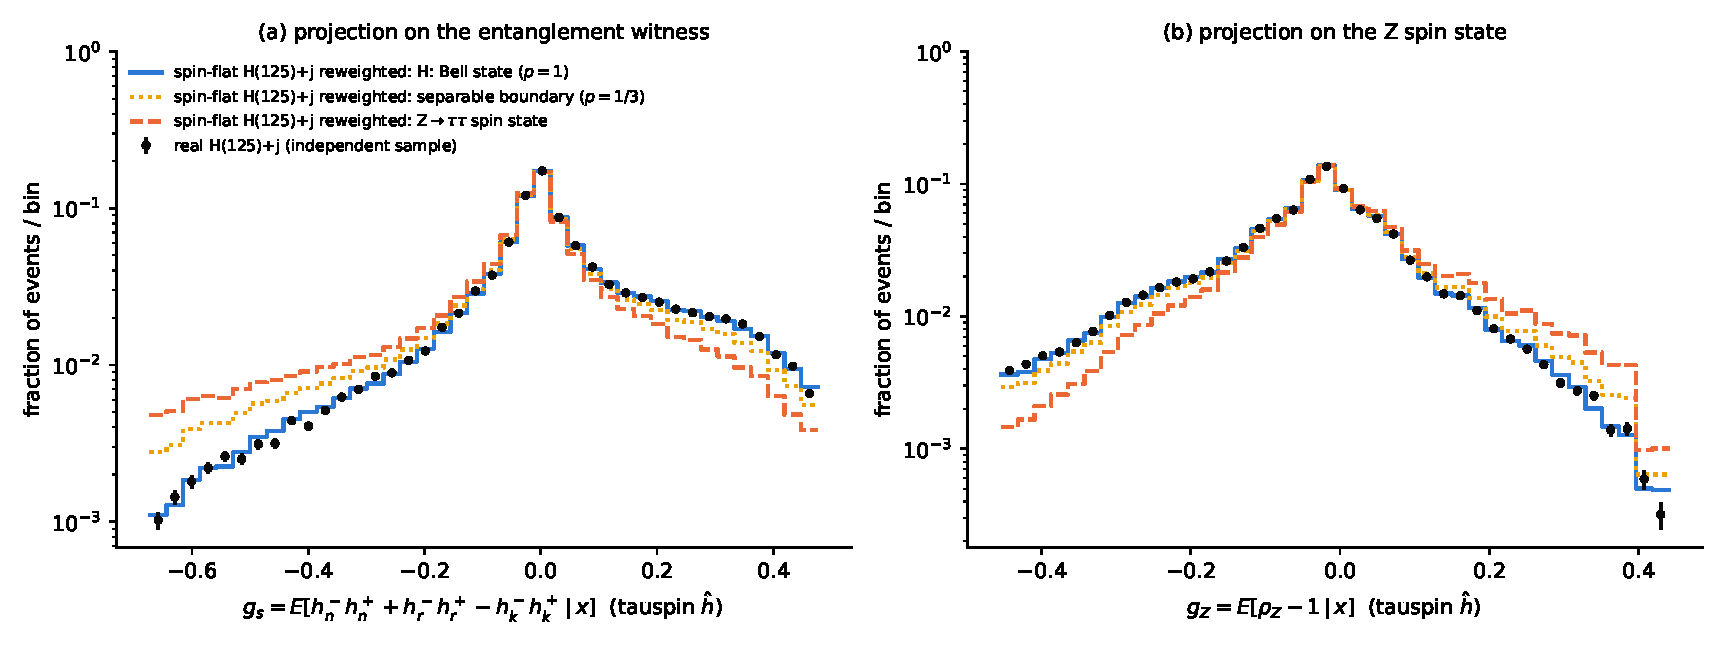
\includegraphics[width=\linewidth]{figures/ent_templates_closure.pdf}
  \caption{スピン平坦な$H(125)$+ジェットを$H$（Bell状態），分離可能な境界（Werner族$p=1/3$），$Z$のスピン状態へ重み付けしたときの統計量の分布と，スピン相関をもつ独立な$H(125)$+ジェット試料（黒点）の比較．(a) もつれのwitnessへの射影，(b) $Z$のスピン状態への射影．どちらの黒点も実際の$H$であり，$H$仮説の分布を再現する．}
  \label{fig:closure}
\end{figure}

\section{解析}\label{sec:ana}

\subsection{HL-LHCの事象数}

信号と背景の事象数は，ATLASの$H\to\tau\tau$断面積測定\cite{ATLAS:2022yrq}の$\tauh\tauh$信号領域12カテゴリ（VBF 2，VH 2，$t\bar tH$ 2，boosted 6）のRun~2の事象数を，$3000/139$倍と14\,TeVの断面積比（信号$1.13$，背景$1.15$）で換算した．各カテゴリを$m_{\tau\tau}$の9ビン（$70$〜$200$\,GeV）に分け，各ビンの信号と背景成分（$Z\to\tau\tau$，fake，top，その他）の割合を本研究のMCで求めた．信号のテンプレートは，各カテゴリの$p_T(\tau\tau)$の範囲の事象から作る（1事象当たりの情報量は$p_T$が大きいほど小さい）．

\subsection{尤度}

カテゴリ$j$，質量ビン$i$，統計量の$6\times6$ビン$b$の期待事象数を
\begin{equation}
  \lambda_{jib}=\mu\,S_{ji}\,T_{jb}(\boldsymbol c;k_T,k_L)+B^{g}_{ji}e^{\alpha^g_{ji}}s^{g}_{jb}+B^{f}_{ji}e^{\alpha^f_{ji}}s^{f}_{jb}
\end{equation}
とする．信号のテンプレート$T_{jb}\propto A_{jb}+k_T(c_nD^n_{jb}+c_rD^r_{jb})+k_Lc_kD^k_{jb}$は，スピン平坦試料のビンごとの和（$A$）と$h^-_ih^+_i$の和（$D^i$）から厳密に作る．$k_T$，$k_L$は横と縦の解析力（真のスピン相関に対する統計量の応答の大きさ）のシミュレーションからのずれを表す係数で，全てのビンに共通である（事前分布$10\%$．$0\%$，$20\%$，$k_T$自由も評価）．

背景は，本物の$\tau$をもつ背景（$Z$，top，その他）とfakeの二つの成分に分け，それぞれの統計量の分布$s^g_j$，$s^f_j$をカテゴリごとに自由なパラメータとする．この分布は9つの質量ビンで共有され，ビンごとの信号と背景の組成の違いから，主に$m_{\tau\tau}$の側帯で決まる（「側帯のみ」）．規格化$\alpha^g$，$\alpha^f$にはそれぞれ$5\%$，$10\%$の事前分布を置く．変種として，信号領域の$r_{\mathrm{aux}}$倍の事象数をもつ補助試料（埋め込み試料やfake因子の対照領域を想定）でこの分布を拘束する場合（$r_{\mathrm{aux}}=0.3$〜$100$）も評価する．データにはAsimovデータを用い，その背景分布には$Z$へ重み付けした分布（本物の$\tau$）と無偏極の分布（fake）を使う．この選択の影響は，背景分布が質量とともに変わる場合も含め，第\ref{sec:res}節の模型誤差の検証で調べる．

もつれの検定統計量は$q=2[\min_{\boldsymbol c\in\mathcal O}\mathrm{NLL}-\min_{\boldsymbol c\in\mathcal T}\mathrm{NLL}]$，期待有意度は$Z=\sqrt q$である（全ての局外パラメータをプロファイル）．CP混合角は，式(\ref{eq:rhophi})のテンプレートで$\varphi=0$のAsimovデータに対する$q(\varphi)$をプロファイルで走査し，小角度での二次近似$q\simeq(\varphi/\sigma_\varphi)^2$から期待精度$\sigma_\varphi$を求める．純CP奇（$\varphi=90^\circ$）の排除は$\sqrt{q(90^\circ)}$で表す．

\section{結果}\label{sec:res}

\begin{figure}[t]
  \centering
  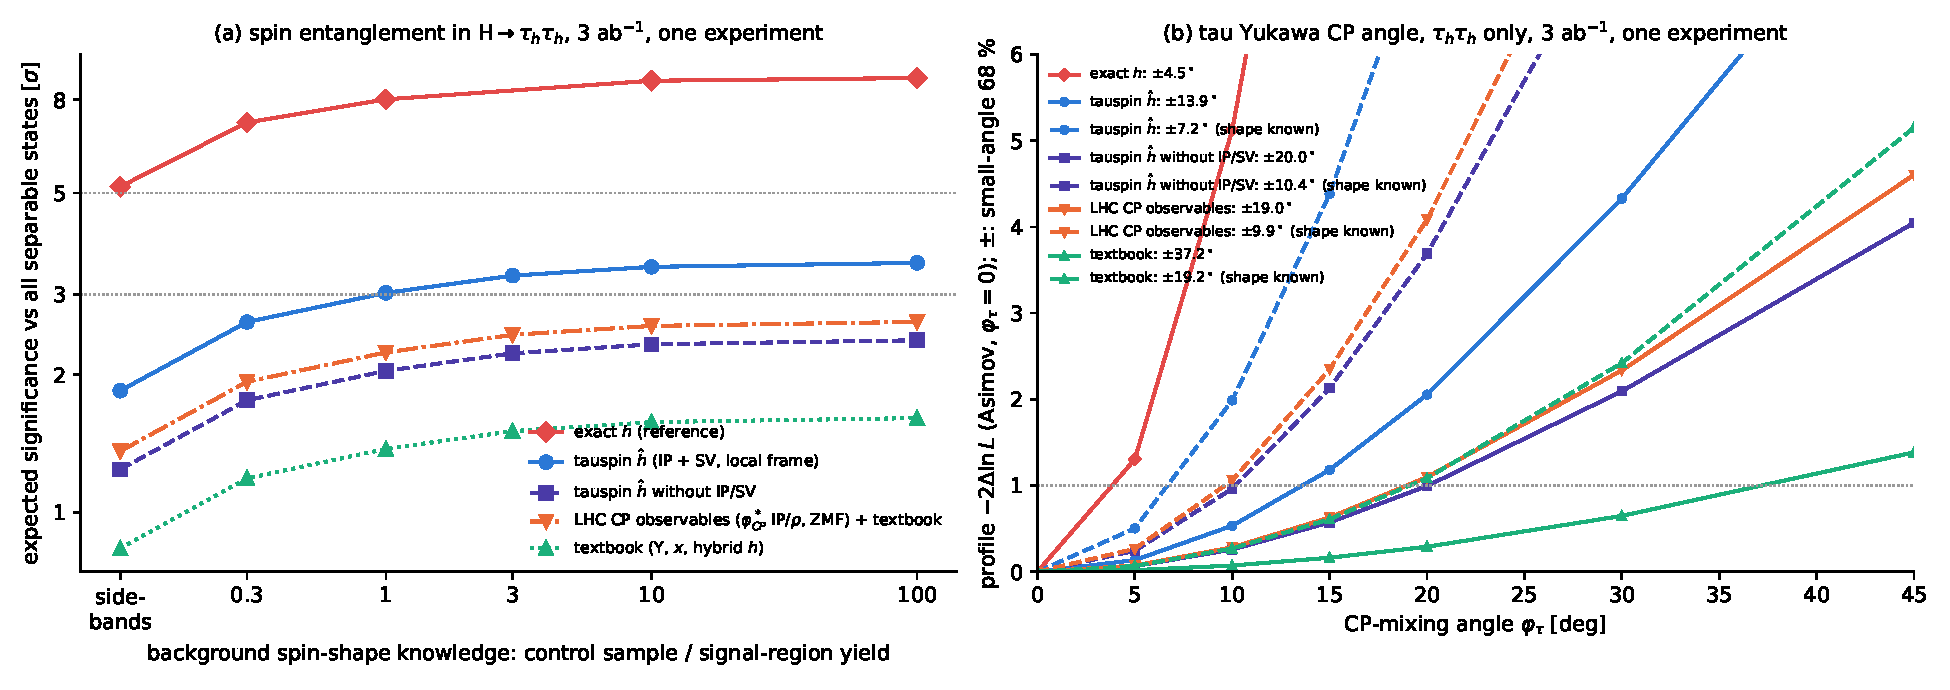
\includegraphics[width=\linewidth]{figures/ent_cp_robust.pdf}
  \caption{HL-LHC（$3\abinv$，1実験，$\tauh\tauh$）での期待感度．(a) 分離可能な全てのBell対角状態に対するもつれの期待有意度と，背景のスピン分布の知識（補助試料の大きさ）の関係．(b) $\tau$湯川結合のCP混合角に対するプロファイル尤度（実線：背景分布を側帯で決める，破線：既知）．凡例の$\pm$は小角度近似での$68\%$の期待精度．}
  \label{fig:main}
\end{figure}

\subsection{もつれ}

\begin{table}[t]
  \centering
  \caption{もつれ（分離可能な全てのBell対角状態の排除）の期待有意度［$\sigma$］，$3\abinv$，1実験．$r_{\mathrm{aux}}$は補助試料の大きさ（信号領域に対する比）．}
  \label{tab:ent}
  \begin{tabular}{lcccccc}
    \toprule
    再構成 & 側帯のみ & $r_{\mathrm{aux}}=0.3$ & $1$ & $3$ & $10$ & 既知（$100$） \\
    \midrule
    正確な$\hvec$ & $5.16$ & $7.13$ & $8.01$ & -- & $8.80$ & $8.92$ \\
    tauspin & $1.84$ & $2.61$ & $3.02$ & $3.29$ & $3.44$ & $3.51$ \\
    tauspin（SV・IP縦・METなし） & $1.81$ & $2.55$ & $2.96$ & $3.23$ & $3.37$ & $3.44$ \\
    tauspin（IP・SVなし） & $1.24$ & $1.76$ & $2.04$ & $2.23$ & $2.33$ & $2.38$ \\
    LHCのCP観測量 & $1.36$ & $1.93$ & $2.24$ & $2.45$ & $2.56$ & $2.61$ \\
    教科書的観測量 & $0.83$ & $1.19$ & $1.38$ & $1.50$ & $1.57$ & $1.61$ \\
    \bottomrule
  \end{tabular}
\end{table}

表\ref{tab:ent}と図\ref{fig:main}(a)に結果を示す．背景のスピン分布を側帯だけで決める場合，tauspinで$1.84\sigma$，LHCのCP観測量で$1.36\sigma$である．信号領域と同じ大きさの補助試料（$r_{\mathrm{aux}}=1$）で分布を拘束すると$3.02\sigma$対$2.24\sigma$，分布が既知なら$3.51\sigma$対$2.61\sigma$となる．どの場合もtauspinの有意度はLHCのCP観測量の$1.35$倍である．倍のルミノシティ（$6\abinv$，同じ尤度の中で局外パラメータを共有）では，tauspinが$2.60/4.23/4.81\sigma$（側帯のみ／$r_{\mathrm{aux}}=1$／$r_{\mathrm{aux}}=10$），LHCのCP観測量が$1.92/3.15/3.59\sigma$である．これはATLASとCMSの結合ではなく，ATLAS型の解析のルミノシティを倍にした場合である．

感度の大部分はVBFの二つのカテゴリ（S/Bの高いVBF\_1で$1.16\sigma$）とboostedカテゴリから来る．帰無仮説の最適点は$\boldsymbol c\approx(0,0.34,-0.66)$にあり，Werner族の一点$p=1/3$を帰無仮説にすると有意度は$2.05\sigma$に上がる（教科書的観測量では$1.33\sigma$で，縦相関に頼る観測量ほどWerner族の仮定で過大評価される）．

\paragraph{解析力の較正の必要性．}横方向の解析力$k_T$を自由にすると，有意度はtauspinでも$0.15\sigma$に落ちる．データの横相関の大きさ$k_T(c_n+c_r)$は，解析力が分からなければ分離可能な状態でも再現できるためである．もつれの主張には，横方向の解析力をシミュレーションと独立に（例えば既知の横相関をもつ過程で）較正する必要がある．$k_T$と$k_L$の事前分布を$0\%$から$20\%$まで変えても結果は$\pm0.02\sigma$しか変わらないので，$10\%$程度で較正できれば十分である．

\subsection{CP混合角}

\begin{table}[t]
  \centering
  \caption{$\tau$湯川結合のCP混合角の期待精度$\sigma_\varphi$［度］（小角度近似，$68\%$），$3\abinv$，1実験．括弧内は純CP奇の排除の期待有意度．}
  \label{tab:cp}
  \begin{tabular}{lcccc}
    \toprule
    再構成 & 側帯のみ & $r_{\mathrm{aux}}=1$ & 既知 & $6\abinv$（側帯のみ） \\
    \midrule
    正確な$\hvec$ & $4.5$ & -- & -- & $3.2$ \\
    tauspin & $13.9$ ($4.0\sigma$) & $8.5$ & $7.2$ ($7.3\sigma$) & $9.9$ \\
    tauspin（SV・IP縦・METなし） & $14.1$ & $8.6$ & $7.3$ & $10.0$ \\
    tauspin（IP・SVなし） & $20.0$ & -- & $10.4$ & $14.2$ \\
    LHCのCP観測量 & $19.0$ ($3.0\sigma$) & $11.5$ & $9.9$ ($5.5\sigma$) & $13.5$ \\
    教科書的観測量 & $37.2$ & -- & $19.2$ & $26.3$ \\
    \bottomrule
  \end{tabular}
\end{table}

表\ref{tab:cp}と図\ref{fig:main}(b)に結果を示す．背景分布を側帯で決める場合，tauspinで$\sigma_\varphi=13.9^\circ$，LHCのCP観測量で$19.0^\circ$，既知なら$7.2^\circ$対$9.9^\circ$である．比は$1.36$〜$1.37$で，もつれの場合（$1.35$）とほぼ同じである．精度はルミノシティの平方根に反比例するので，同じ精度を得るのに必要なルミノシティは約$1.9$分の1になる．

CP混合角は横相関の「回転」の測定なので，解析力の全体スケール$k_T$を自由にしても小角度の精度は$13.9^\circ\to14.7^\circ$とほとんど変わらない（ただし純CP奇の排除と$95\%$区間は$k_T$に依存する）．CP奇成分（$\sin2\varphi$の項）に別の応答$k_A$を与えると，事前分布$10\%$では$14.0^\circ$で変わらないが，自由にすると局所的な精度が失われる（約$45^\circ$）．$\varphi_\tau$の測定には，CP偶とCP奇の成分の解析力の相対的な較正（$10\%$程度）が必要である．

\subsection{頑健性の検証}

\begin{itemize}
  \item \textbf{偽陽性．}分離可能な状態（帰無仮説の最適点）を信号として注入すると，有意度は全ての再構成水準で$0.00\sigma$である．
  \item \textbf{背景の模型誤差．}本物の$\tau$の背景のスピン分布が，$m_{\tau\tau}$の低い側の$Z$偏極から高い側の無偏極へ連続的に変わる（尤度で表せない）とすると，分離可能な状態の注入による偽の有意度はtauspinで$0.40\sigma$，LHCのCP観測量で$0.38\sigma$，教科書的観測量で$0.24\sigma$である．背景の運動学が$H$+ジェットから実際の$Z(125)$+ジェットへ変わる場合，偽の有意度は$0.18\sigma$（教科書的観測量では$0.84\sigma$）で，真の$H$信号の有意度は$0.55\sigma$に下がる．背景の分布が質量に強く依存すると感度は失われるが，偽のもつれは生じにくい．
  \item \textbf{ビン分割．}統計量のビンを$4\times4$，$8\times8$にすると，tauspinで$1.68$，$1.93\sigma$，LHCのCP観測量で$1.24$，$1.42\sigma$（側帯のみ）であり，比は変わらない．
  \item \textbf{テンプレートのMC統計．}背景分布を既知とした簡略な尤度で，テンプレートを試料の半分ずつから作ると$3.74$，$3.84\sigma$（全体で$3.78\sigma$），ブートストラップのばらつきは$\pm0.03\sigma$であった．テンプレートのMC統計による偏りは小さい．本論文の尤度では背景のテンプレートをMCから取らないので，この寄与はさらに小さいと考えられるが，同じ検証は行っていない．
  \item \textbf{高S/Bのカテゴリのみ．}S/Bが$5\%$を超えるカテゴリだけでも，tauspin $1.21\sigma$，LHCのCP観測量$0.87\sigma$で，比は保たれる．
\end{itemize}

\section{議論}\label{sec:disc}

\paragraph{比と絶対値．}本論文の確かな結論は，同じ枠組みの中での再構成水準の間の比である．絶対値は解析の設定に強く依存する．同じ枠組みのLHCのCP観測量を$139\fbinv$に適用すると，側帯のみの尤度では$q(90^\circ)=0.36$で$68\%$の区間すら得られない．背景分布既知の結果をルミノシティで外挿しても約$\pm49^\circ$であり，ATLASのRun~2の期待精度$\pm28^\circ$（全チャンネル）より約1.7倍悪い（側帯のみの尤度ではさらに悪い）．主な理由は，$\tauh\tauh$のみであること，ATLASの断面積測定のカットベースのカテゴリを使っていること，背景の分布をデータで決めていることである．HL-LHCの$\varphi_\tau$の既存の投影（約$\pm5$〜$8^\circ$\cite{HiggsHLLHC}）にtauspinの利得の比を当てはめると，同じ精度に必要なルミノシティが約半分になる，あるいは精度が約$1/1.37$になることが期待されるが，これは比の移転であり独立な投影ではない．

\paragraph{もつれの主張の範囲．}1実験・HL-LHCで，分離可能な全てのBell対角状態を$5\sigma$で排除するのは難しい．背景分布を補助試料で拘束し（$r_{\mathrm{aux}}\gtrsim1$），横方向の解析力を独立に較正したうえで，1実験で約$3\sigma$，倍のルミノシティで$4$〜$5\sigma$が見込める．帰無仮説はBell対角状態に限っており，偏極や非対角の相関をもつ分離可能な状態は含めていない（CP偶の$H$のデータに対しては影響は小さいと考えられるが確かめていない）．

\paragraph{比較の公平性．}LHCのCP観測量の基準は，ATLASの3本トラックの崩壊面の方法やCMSの$a_1$偏極計による扱いより弱い．また，tauspinの側は専用のニューラルネットワーク，比較対象の側は勾配ブースティングという違いがあり，同じ入力の生の値に勾配ブースティングを当てると横相関の統計量の相関は$0.11$にしかならなかった．したがって本論文の利得は「横方向のIPの情報」と「それを学習した偏極計で使うこと」を合わせた手法としての利得であり，情報量だけの主張ではない．

\paragraph{未評価の系統．}IP・SVの分解能の変化（$1.3$倍など）や非ガウス型の裾，$\pi^0$のエネルギー較正，$\tau$崩壊模型の変動，$\taul\tauh$チャンネル，ATLASとCMSの結合は評価していない．補助試料は真の分布を誤差なく測ると仮定しており，その移転の不確かさは入れていない．

\section{結論}\label{sec:concl}

学習した$\tau$偏極計（tauspin）を用いて，HL-LHCでの$H\to\tau\tau$のスピン状態の測定感度を，$\tau$湯川結合のCP混合角と$\tau$対のスピンもつれについて見積もった．背景のスピン分布をデータで決め，帰無仮説を分離可能な全ての状態にとる頑健な尤度のもとで，tauspinはLHCのCP解析の観測量を最適に組み合わせたものに対し，CP混合角の精度ともつれの有意度の両方で一貫して$1.35$〜$1.37$倍（ルミノシティ換算で約$1.8$〜$1.9$倍）の感度を与える．この利得の大部分は横方向のIPに由来し，SV，IPの縦成分，欠損運動量は寄与しない．1実験・$3\abinv$で，CP混合角の期待精度は$\pm13.9^\circ$（背景分布を側帯で決める場合）から$\pm7.2^\circ$（既知の場合），もつれの期待有意度は$1.8\sigma$から$3.5\sigma$である．もつれの確立には背景分布の補助的な拘束と横方向の解析力の独立な較正が必要であり，CP混合角の測定は解析力の全体スケールに頑健である．

\section*{謝辞}
計算にはICEPPの計算機資源を用いた．

\appendix
\section{$\phicp$の構成}\label{app:phicp}

各$\tau$について四元ベクトルの対$(q,\lambda)$を選ぶ．$\pi^0$を伴わない1本トラックと3本トラックの崩壊では，$q$を先頭の荷電トラック，$\lambda=(0,\boldsymbol d)$をそのPV基準のIPベクトルとする（IP法）．$\pi^0$を伴う崩壊では，$q$を荷電パイオン，$\lambda$を$\pi^0$の和とする（$\rho$法）．二つの$q$の零運動量系へ全てをブーストし，$\lambda$の$q$に垂直な成分を規格化して$\hat\lambda^\pm_\perp$とする．$\phicp=\arccos(\hat\lambda^+_\perp\cdot\hat\lambda^-_\perp)$とし，$\hat q^-\cdot(\hat\lambda^+_\perp\times\hat\lambda^-_\perp)<0$なら$2\pi-\phicp$とする．$\rho$法の側の$y$の積が負なら$\pi$ずらす．

\begin{thebibliography}{99}
\bibitem{ATLAS:2022akr} ATLAS Collaboration, ``Measurement of the $CP$ properties of Higgs boson interactions with $\tau$-leptons with the ATLAS detector,'' Eur.\ Phys.\ J.\ C \textbf{83} (2023) 563, arXiv:2212.05833.
\bibitem{CMS:2021sdq} CMS Collaboration, ``Analysis of the $CP$ structure of the Yukawa coupling between the Higgs boson and $\tau$ leptons in proton-proton collisions at $\sqrt s=13$ TeV,'' JHEP \textbf{06} (2022) 012, arXiv:2110.04836.
\bibitem{Berge:2008dr} S.~Berge, W.~Bernreuther and J.~Ziethe, ``Determining the CP parity of Higgs bosons at the LHC in their tau decay channels,'' Phys.\ Rev.\ Lett.\ \textbf{100} (2008) 171605, arXiv:0801.2297.
\bibitem{Berge:2015nua} S.~Berge, W.~Bernreuther and S.~Kirchner, ``Prospects of constraining the Higgs boson's CP nature in the tau decay channel at the LHC,'' Phys.\ Rev.\ D \textbf{92} (2015) 096012, arXiv:1510.03850.
\bibitem{ATLAS:2023fsd} ATLAS Collaboration, ``Observation of quantum entanglement with top quarks at the ATLAS detector,'' Nature \textbf{633} (2024) 542, arXiv:2311.07288.
\bibitem{CMS:2024pts} CMS Collaboration, ``Observation of quantum entanglement in top quark pair production in proton-proton collisions at $\sqrt s=13$ TeV,'' Rep.\ Prog.\ Phys.\ \textbf{87} (2024) 117801, arXiv:2406.03976.
\bibitem{Afik:2020onf} Y.~Afik and J.~R.~M.~de Nova, ``Entanglement and quantum tomography with top quarks at the LHC,'' Eur.\ Phys.\ J.\ Plus \textbf{136} (2021) 907, arXiv:2003.02280.
\bibitem{Altakach:2022ywa} M.~M.~Altakach, P.~Lamba, F.~Maltoni, K.~Mawatari and K.~Sakurai, ``Quantum information and CP measurement in $H\to\tau^+\tau^-$ at future lepton colliders,'' Phys.\ Rev.\ D \textbf{107} (2023) 093002, arXiv:2211.10513.
\bibitem{Fabbrichesi:2022ovb} M.~Fabbrichesi, R.~Floreanini and E.~Gabrielli, ``Constraining new physics in entangled two-qubit systems: top-quark, tau-lepton and photon pairs,'' Eur.\ Phys.\ J.\ C \textbf{83} (2023) 162, arXiv:2208.11723.
\bibitem{Ma:2023yvd} K.~Ma and T.~Li, ``Testing Bell inequality through $h\to\tau\tau$ at CEPC,'' arXiv:2309.08103.
\bibitem{QI:ESPPU} Y.~Afik \textit{et al.}, ``Quantum information meets high-energy physics: input to the update of the European Strategy for Particle Physics,'' arXiv:2504.00086.
\bibitem{ZttEnt} Zhang \textit{et al.}, arXiv:2504.01496.
\bibitem{Hagiwara:2016zqz} K.~Hagiwara, K.~Ma and S.~Mori, ``Probing CP violation in $h\to\tau^-\tau^+$ at the LHC,'' Phys.\ Rev.\ Lett.\ \textbf{118} (2017) 171802, arXiv:1609.00943.
\bibitem{HtautauCPV} Chen and Wu, ``Probing the CP-violation effects in the $h\tau\tau$ coupling at the LHC,'' arXiv:1708.02882.
\bibitem{Jozefowicz:2016kvz} R.~Józefowicz, E.~Richter-Wąs and Z.~Wąs, ``Potential for optimizing the Higgs boson CP measurement in $H\to\tau\tau$ decays at the LHC including machine learning techniques,'' Phys.\ Rev.\ D \textbf{94} (2016) 093001, arXiv:1608.02609.
\bibitem{Lasocha:2020ctd} K.~Lasocha, E.~Richter-Wąs, D.~Tracz, Z.~Wąs and P.~Winkowska, ``Deep neural network application: Higgs boson CP state mixing angle in $H\to\tau\tau$ decay and at the LHC,'' arXiv:2001.00455.
\bibitem{Lasocha:2024} E.~Richter-Wąs \textit{et al.}, ``Pseudo-observables and deep neural network for mixed CP $H\to\tau\tau$ decays at LHC,'' arXiv:2411.06216.
\bibitem{Horodecki:1996} R.~Horodecki and M.~Horodecki, ``Information-theoretic aspects of inseparability of mixed states,'' Phys.\ Rev.\ A \textbf{54} (1996) 1838.
\bibitem{Peres:1996dw} A.~Peres, ``Separability criterion for density matrices,'' Phys.\ Rev.\ Lett.\ \textbf{77} (1996) 1413.
\bibitem{Werner:1989zz} R.~F.~Werner, ``Quantum states with Einstein-Podolsky-Rosen correlations admitting a hidden-variable model,'' Phys.\ Rev.\ A \textbf{40} (1989) 4277.
\bibitem{Abel:2025} S.~Abel \textit{et al.}, arXiv:2507.15949.
\bibitem{Bechtle:2025} P.~Bechtle \textit{et al.}, arXiv:2507.15947.
\bibitem{Bierlich:2022pfr} C.~Bierlich \textit{et al.}, ``A comprehensive guide to the physics and usage of PYTHIA 8.3,'' SciPost Phys.\ Codeb.\ \textbf{2022} (2022) 8, arXiv:2203.11601.
\bibitem{Czyczula:2012ny} Z.~Czyczula, T.~Przedzinski and Z.~Was, ``TauSpinner program for studies on spin effect in tau production at the LHC,'' Eur.\ Phys.\ J.\ C \textbf{72} (2012) 1988, arXiv:1201.0117.
\bibitem{dihiggs:paper} 著者ら，「$\tau$レプトンのスピンと寿命の情報によるHL-LHCでの$HH\to b\bar b\tau^+\tau^-$探索感度の改善の見積もり」（姉妹論文）．
\bibitem{Pedregosa:2011} F.~Pedregosa \textit{et al.}, ``Scikit-learn: Machine learning in Python,'' J.\ Mach.\ Learn.\ Res.\ \textbf{12} (2011) 2825.
\bibitem{Elagin:2010aw} A.~Elagin, P.~Murat, A.~Pranko and A.~Safonov, ``A new mass reconstruction technique for resonances decaying to $\tau\tau$,'' Nucl.\ Instrum.\ Meth.\ A \textbf{654} (2011) 481, arXiv:1012.4686.
\bibitem{ATLAS:2022yrq} ATLAS Collaboration, ``Measurements of Higgs boson production cross-sections in the $H\to\tau^+\tau^-$ decay channel in $pp$ collisions at $\sqrt s=13$ TeV with the ATLAS detector,'' JHEP \textbf{08} (2022) 175, arXiv:2201.08269.
\bibitem{HiggsHLLHC} M.~Mlynarikova, ``Higgs physics at the HL-LHC,'' arXiv:2307.07772.
\end{thebibliography}

\end{document}
